\documentclass[bachelor, och, labwork]{shiza}

\usepackage[utf8]{inputenc}
\usepackage{graphicx}

\usepackage[sort,compress]{cite}
\usepackage{amsmath}
\usepackage{amssymb}
\usepackage{amsthm}
\usepackage{fancyvrb}
\usepackage{longtable}
\usepackage{array}
\usepackage[english,russian]{babel}
\usepackage{minted}

\usepackage{tempora}


% \usepackage[colorlinks=false]{hyperref}


\newcommand{\eqdef}{\stackrel {\rm def}{=}}


\begin{document}

\title{Алгоритмы алгебры и теории чисел}

\course{4}

\group{431}

\napravlenie{10.05.01 "--- Компьютерная безопасность}


\author{Никитина Арсения Владимировича}


\satitle{доцент}
\saname{А.\,С.\,Гераськин}


\date{2022}

\maketitle

% Включение нумерации рисунков, формул и таблиц по разделам
% (по умолчанию - нумерация сквозная)
% (допускается оба вида нумерации)
%\secNumbering


\tableofcontents

\section{Задание лабораторной работы}

Разложение на мнодители полиномов над конечными полями:

\begin{itemize}
    \item Алгоритм Бэрликемпа.
\end{itemize}

\section{Теоретическая часть}

\begin{center}
    \textit{Разложение полиномов на свободные от квадратов мно-
множители (Polynomial Squarefree Factorization)}
\end{center}

\textit{Вход:} Нормированный свободный от квадратов полином $p(x)$ над $GF(p),\\
\deg [p(x)]= n.$

\textit{Выход:} Неприводимые сомножители полинома $p(x)$ над $GF(p)$.

\begin{enumerate}
   \item Построить матрицу $Q$ размерности $n \times n$. 
   \item Триангулировать матрицу $Q-I$, вычислив ее ранг $n-r$ и найдя нуль-пространство
   матрицы $Q-I$, то есть найти $r$ линейно независимых векторов $b_1, \dots, b_r$,
   таких, что $b_j[Q-I]=0, j=\overline{1, r}$. Первый вектор всегда может быть
   выбран в виде $\left(1, 0, \dots, 0\right)$, что представляет тривиальное
   решение $b_1(x)=1$ уравнения.
   \item Вычисление сомножителей. Пусть $b_2(x)$ --- полином, соответствующий
   вектору $b_2$. Вычислим $\gcd(p(x), b_2(x)-s) ~ \forall s \in GF(p).$
   В результате данной операции будет получено нетриваиельное разложение
   полинома $p(x)$. Если с использованием $b_2(x)$ получено менее $r$ сомножителей,
   вычислим $\gcd(w(x), b_k(x) - s) ~\forall s \in GF(p)$ и для всех сомножителей
   $w(x)$, найденных к данному времений для $k = \overline{3, r}$, пока не будет
   найдено $r$ сомножителей. Таким образом гарантируется, что будут найдены все
   сомножители полинома $p(x)$. Если $p$ достаточно мало, то вычисления на данном
   шаге можно считать эффективными. Считается, что если $p > 25$, следует
   использовать более эффективные алгоритмы.
\end{enumerate}


\section{Практическая часть}
\subsection{Пример работы алгоритма}
\begin{figure}[H]
    \centering
    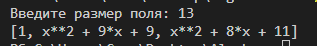
\includegraphics[width=1\textwidth]{pic1.png}
    \caption{}
\end{figure}


\setminted[python]{linenos,breaklines=true, fontsize=\small, style=bw}
    \subsection{Код программы, реализующей рассмотренный алгоритм}
        \inputminted{python}{lab18.py}


\end{document}